\section{Slice Helper Functions}

\subsection{Choosing the functions}

The first task is to implement some helper functions for slices, as they are present
for lists in Haskell. To decide on which functions will be implemented, popular
Haskell repositories on Github have been analysed. The popularity of repositories
was decided to be based on their number of stars. Out of all Haskell projects
on Github, the most popular are\autocite{github-popular-haskell}:

\begin{itemize}
    \item Shellcheck (koalaman/shellcheck\autocite{github-shellcheck}): A static analysis tool for shell scripts
    \item Pandoc (jgm/pandoc\autocite{github-pandoc}): A universal markup converter
    \item Postgrest (PostgREST/postgrest\autocite{github-postgrest}): REST API for any Postgres database
    \item Semantic (github/semantic\autocite{github-semantic}): Parsing, analyzing, and comparing source code across many languages
    \item Purescript (purescript/purescript\autocite{github-purescript}): A strongly-typed language that compiles to JavaScript
    \item Compiler (elm/compiler\autocite{github-elmcompiler}): Compiler for Elm, a functional language for reliable webapps
    \item Haxl (facebook/haxl\autocite{github-haxl}): A Haskell library that simplifies access to remote data, such as databases or web-based services
\end{itemize}

In these repositories, the number of occurrences of popular list functions have
been counted. The analysis does not differentiate between different kind of
functions. For example, `fold' includes all occurrences of `foldr', `foldl' and
`foldl\''. Also, the analysis has not been done with any kind of AST-parsing.
Rather, a simple `grep' has been used to find matches. This means that it is
likely to contain some mismatches, for example in code comments. All in all,
this analysis should only be an indicator of what functions are used most.

 % TODO: replace 'prepend' with cons, where applicable (talking about Haskell)
Running the analysis on the 7 repositories listed above, searching for a number
of pre-selected list functions, indicates that the most used functions are `:'
(cons), `map' and `fold', as shown in table~\ref{tab:occurrences-list-funcs}.

\begin{table}[htb]
\centering
\caption{Occurrences of list functions\ref{appendix:function-occurrences}}\label{tab:occurrences-list-funcs}
\begin{tabular}{ll}
\toprule
map & 1241 \\
\midrule
`:' (cons) & 1177 \\
\midrule
fold & 610 \\
\midrule
filter & 262 \\
\midrule
reverse & 154 \\
\midrule
take & 104 \\
\midrule
drop & 81 \\
\midrule
maximum & 53 \\
\midrule
sum & 44 \\
\midrule
zip & 38 \\
\midrule
product & 15 \\
\midrule
minimum & 10 \\
\midrule
reduce & 8
\end{tabular}
\end{table}
\footnote{The cons function (`:') is overrepresented in this list,
    as it can also be used to deconstruct lists within pattern matching. Filtering
    these occurrences would need a more advanced algorithm. However, even if $\tfrac{3}{4}$
    of these usages are used in pattern matching, the cons function would still be
    in the top 3.
}
\footnote{The map function listed here also includes occurrences of `fmap'. A more
    detailed look at the data shows that there are 632 occurrences of `fmap', which
    means that `fmap' and `map' are used equally as often. As `fmap' however requires
    some kind of implementation for an `iterable', it is out of scope for this paper.
}

Based on this information, it has been decided to implement the map, cons, fold
and filter functions into the Go compiler.

\subsection{The Go Compiler}

The Go programming language is defined by its specification\autocite{go-spec}, and not
it's implementation. As of Go 1.14, there are two major implementations of that
specification; Google's self-hosting compiler toolchain\footnote{This is what most
    often is referred to as `the Go compiler'.}
`gc', which is written in Go, and `gccgo', a frontend for GCC, writen in C++.

When talking about the Go compiler, what's mostly referred to is `gc'\footnote{`gc' stands
for `Go Compiler', and not `Garbage Collection' (`GC').}.

A famous, although not completely correct story tells about Go being designed
while a C++ program was compiling\autocite{less-is-more}.
This is why one of the main goals when designing Go was fast compilation times:
\begin{quote}
    Finally, working with Go is intended to be fast: it should take at most a few
    seconds to build a large executable on a single computer. To meet these goals
    required addressing a number of linguistic issues: an expressive but lightweight
    type system; concurrency and garbage collection; rigid dependency specification;
    and so on. These cannot be addressed well by libraries or tools; a new language
    was called for.\autocite{go-faq}
\end{quote}

This is why Go has taken some measures to to combat slow compilation times. According
to Rob Pike, one of the creators of Go, Go's compiler is not notably fast, but
most other compilers are slow:

\begin{quote}
    The compiler hasn't even been properly tuned for speed. A truly fast compiler
    would generate the same quality code much faster.\autocite{nuts-compiler}
\end{quote}

The language design does have some limitations
however to lower compilation times. In general, Go's dependency resolution is simpler
compared to other languages, for example by not allowing circular dependencies.
Furthermore, compilation is not even attempted if there are unused
imports or unused declarations of variables, types and functions.
This leads to less code to compile and in turn shorter compilation times.
Another reason is that `the `gc' compiler is simpler code compared to most
recent compilers'\autocite{nuts-compiler}.

Compiling Go programs with the standard `gc' compiler can be split into four
phases:

\subsubsection{Parsing Go programs}

\newglossaryentry{dag}{name=DAG, description={Directed Acyclic Graph}}
\newglossaryentry{ast}{name=AST,description={Abstract Syntax Tree, an abstract representation of source code as a tree}}

The first phase of compilation is parsing Go programs into a syntax tree. This
is done by tokenizing the code (`lexical analysis' - the `lexer'), parsing
(`syntax analysis' - the `parser') it and then constructing a syntax tree (\gls{ast}) for
each source file\footnote{Technically, the syntax tree is a syntax \gls{dag}\autocite{ast-node-dag}}.

In comparison to most production-level languages, Go can be parsed without a
symbol table. It has been designed to be easy to parse
and analyse, which makes the Go parser simple in it's design\autocite{go-faq-symbol}.

\subsubsection{Type-checking and AST-transformation}\label{sec:comp-type}

The second phase of compilation starts by converting the `syntax' package's
AST, created in the first phase, to the compiler's AST representation. This
is due to historical reasons, as the `gc's AST definition was carried over
from the C implemenation.

After the conversion, the AST is type-checked. Within the type-checking, there
are also some additional steps included like `declared and not used' and
determining wheter a function terminates.

After type-checking, some transformations are applied on the AST. This includes,
but is not limited to, eliminating dead code, inlining function calls and escape
analysis. What is also done in the transformation phase is rewriting builtin function
calls, replacing for example a call to the builtin `append' with the necessary
AST structure and rutime-calls to implement its functionality.

\subsubsection{SSA}

\newglossaryentry{ssa}{name=SSA,description={Single Static Assignment, an intermediate representation between the AST and the compiled binary that simplifies and improves compiler optimisations}}
In the third phase, the AST is converted to \gls{ssa} form. SSA  is `a
lower-level intermediate representation with specific properties that make it
easier to implement optimizations and to eventually generate machine code from
it'\autocite{compiler-readme}.

The conversion consists of multiple `passes' through the SSA that
apply machine-independent rules to optimise code. These generic
rewrite rules are applied on every architecture and thus mostly
concern expressions (e.g. replace expressions with constant values and
optimise multiplications), dead code elimination and removal of unneeded
nil-checks.

\subsubsection{Generating machine code}

Lastly, in the fourth phase of the compilation, machine-specific
SSA optimisations are applied, including, but not limited to:
\begin{itemize}
    \item Rewriting generic values into their machine-specific variants
        (for example, on amd64, combining load-store operations)
    \item Another dead-code elimination pass
    \item Pointer liveness analysis
    \item Removing unused local variables
\end{itemize}

After generating and optimising the SSA form, the code is passed to the
assembler, which replaces the so far generic instructions with
architecture-specific machine code and writes out the final object file.
\autocite{compiler-readme}

\subsection{Built-in functions}

What has only been discussed very briefly in chapter \ref{sec:comp-type} are
built-in functions. The language specification defines what built-in functions
are and which built-in functions should exist:
\begin{quote}
    Built-in functions are predeclared. They are called like any other function
    but some of them accept a type instead of an expression as the first argument.

    The built-in functions do not have standard Go types, so they can only appear
    in call expressions; they cannot be used as function values.\autocite{go-spec-builtins}
\end{quote}

As Go does not have generics (polymorphism), functions that return a variable but
concrete type have to be built-in into the language itself.

For example, if `append' would not exist as a built-in, there would be two options
to work around that.

One option would be that `append' would take and return empty interfaces
(\mintinline{go}|interface{}|). However, `the empty interface says
nothing'\autocite{empty-interface}. The declaration of `append' would be:
\begin{gocode}
  func append(slice []interface{}, elem ...interface{}) {}interface
\end{gocode}

This function header does not say anything about it's types, which would
mean that they would need to be checked at runtime and handled gracefully. It
would also require the caller to do a type assertion after every call:

\begin{gocode}
  s := []string{"hello"}
  s = append(s, "world").([]string)
\end{gocode}

It also does not specify that the slice's element type would need to be equal to
the appended element. Instead, this would need to be a convention.

The other option would be to specify a function upon each type, meaning:
\begin{gocode}
func appendInt(slice []int, elem ...int} []int
func appendString(slice []string, elem ...string} []string
...
\end{gocode}

Which is not only extremely verbose, but also misses any custom user-defined types.

For this reason, the helper function that should  be implemented need to
be implemented within the compiler, as built-in functions.

\subsection{Map}

The most used function in Haskell is map. The table \ref{tab:occurrences-list-funcs}
counts ~1200 occurrences of map, although ~600 of those occurrences are from
fmap. fmap is the generic version of map: while map only works on lists, fmap
works on every type that implements the `Functor' typeclass\footnote{typeclasses
    in Haskell are what would be interfaces in imperative and object-oriented
languages}, including tuples, `Maybe' and lists.
`In practice a functor represents a type that can be mapped over.'\autocite{functor-wiki}
A common analogy for functors are `boxes'. A functor behaves like a box where
a value can be put into and taken out again. For lists, the operation of `taking out'
elements means processing each value one by one. For `Maybe', it means `unpacking' the
concrete value and processing it, and if there is no concrete value, returning `Nothing'
instead.

map (and fmap) is one of the most useful higher-order functions:
\begin{quote}
    \[map\] returns a list constructed by appling a function (the first argument) to all
    items in a list passed as the second argument\autocite{haskell-map}.
\end{quote}

Some usage examples of map can be found at~\ref{code:haskell-map}.

\begin{code}
    \captionof{listing}{Example usage for map and fmap}
    \label{code:haskell-map}
    \begin{haskellcode}
Prelude> :t map
map :: (a -> b) -> [a] -> [b]
Prelude> :t fmap
fmap :: Functor f => (a -> b) -> f a -> f b
Prelude> map (*3) [1,2,3]
[3,6,9]
Prelude> fmap (*3) [1,2,3]
[3,6,9]
Prelude> map (++ " world") ["hello","goodbye"]
["hello world","goodbye world"]
Prelude> map show [1,2,3]
["1","2","3"]
    \end{haskellcode}
\end{code}

Due to missing polymorphism, map cannot be implemented as easily in Go. While
a specific definition of map would be
\mintinline{go}|func map(f func(int) string, []int) []string|,
this definition would only hold true for the specific types \mintinline{go}|int|
and \mintinline{go}|string|. A more generic definition, similar to append,
would be \mintinline{go}|func map(f func(Type1) Type2, []Type1) []Type2|. For
this to work, the function has to be implemented as a builtin into the compiler.

As there is already a `map' token in the Go compiler (for the map data type),
the function will be called `fmap'. However, compared to Haskell's `fmap',
Go's `fmap' only works on slices. This is due
to the absence of an `iterator'-like concept. The `range' clause, used with
`for' loops, only works on slices and maps - both are builtin data types. It does
not work on custom data structures, which would make the implementation a far
bigger task.
Nonetheless, to avoid possible naming confusions, the `map' function in Go will
be called `fmap'.

In Go, the usage of `fmap' should result in making the program \ref{code:fmap-usage-go}
behave as shown.

\begin{code}
    \captionof{listing}{Example usage of map in go}
    \label{code:fmap-usage-go}
    \begin{gocode}
package main

import (
  "fmt"
  "strconv"
)

func main() {
  fmt.Printf("%#v", fmap(strconv.Itoa, []int{1, 2, 3})) // []string{"1", "2", "3"}
}
\end{gocode}
\footnote{Printf's first argument, the verb `\%\#v', can be used to print the type
(`\#') and the value (`v') of a variable\autocite{fmt-godoc}.}
\end{code}

\subsection{Cons}

The name cons has been introduced by LISP, where it describes a record structure
containing two components called the `car' (the `contents of the address register'),
and the `cdr' (`content of decrement register').
Lists are built upon cons cells, where the `car' stores the element and `cdr' a
pointer to the next cell - the next element of the list.
This is why in Lisp, \mintinline{lisp}|(cons 1 (cons 2 (cons 3 (cons 4 nil))))| is equal to
\mintinline{lisp}|(list 1 2 3 4)|. This list is also visualised in picture~\ref{fig:cons}.

\begin{figure}[h!]
  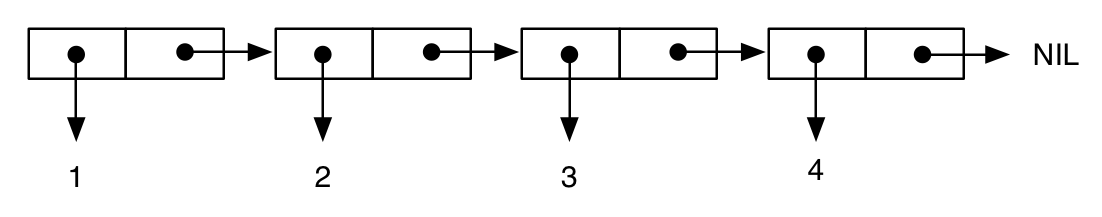
\includegraphics[width=\linewidth]{../img/cons.png}
  \caption{Cons cells forming a list\autocite{cons-image-source}}
  \label{fig:cons}
\end{figure}

The cons operator thus prepends an element to a list, effectively allocating a
variable that contains the newly added element and a pointer to the `old' list.
As a result, prepending to a list is computationally cheap, needing one allocation
and one update.

In Haskell, the `name' of the cons function is the `:' operator.
In Go, names for identifiers (which includes function names) underlie a simple
rule:
\begin{quote}
    An identifier is a sequence of one or more letters and digits. The first
    character in an identifier must be a letter.\autocite{spec-identifiers}
\end{quote}

This rule forbids a function to be named `:'. Instead, the function could be
named `cons'. However, Go already has a function to add to the end of a slice,
`append'. Thus, adding to the beginning of a slice will be named `prepend'.
Using prepend is very similar to append, an example can be found at~\ref{code:prepend-go}

\begin{code}
    \captionof{listing}{Example usage of prepend in go}
    \label{code:prepend-go}
    \begin{gocode}
package main

import (
  "fmt"
  "strconv"
)

func main() {
    fmt.Printf("%#v", prepend(0, []int{1, 2, 3})) // []int{0, 1, 2, 3}
}
\end{gocode}
\end{code}

\subsection{Fold}\label{sec:fold}

Fold, sometimes also named `reduce' or `aggregate' is another higher-order function
that is very commonly used in functional programming.

\begin{quote}
    analyze a recursive data structure and through use of a given
    combining operation, recombine the results of recursively processing its
    constituent parts, building up a return value.\autocite{fold-wiki}
\end{quote}

The family of fold functions in Haskell consist of three different implementations of
that definition: `foldr', `foldl' and `foldl\''.
The difference between foldr and foldl is hinted at their function headers:
\begin{code}
    \captionof{listing}{Function headers of the fold functions}
    \begin{haskellcode}
Prelude Data.List> :t foldr
foldr :: Foldable t => (a -> b -> b) -> b -> t a -> b
Prelude Data.List> :t foldl
foldl :: Foldable t => (b -> a -> b) -> b -> t a -> b
    \end{haskellcode}
\end{code}

The argument with type `b' is passed as the first argument to the foldl
function, and as the second argument to foldr. As can be seen in the illustrations
of foldl and foldr in~\ref{fig:fold}, the evaluation order of the two functions
differ.

\begin{figure}[h!]
    \centering
    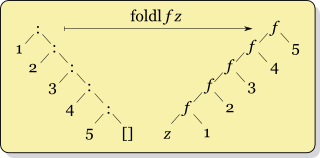
\includegraphics[scale=0.5]{../img/foldl.png}
    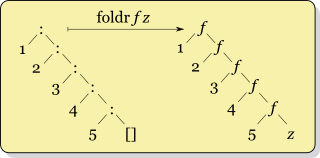
\includegraphics[scale=0.5]{../img/foldr.png}
    \caption{Folds illustrated\autocite{fold-wiki}}
    \label{fig:fold}
\end{figure}

This is most obvious when using an example where the function is not associative:

\begin{code}
    \captionof{listing}{foldr and foldl execution order}
    \label{code:foldr-example}
    \begin{haskellcode}
foldr (-) 0 [1..7]
1 - (2 - (3 - (4 - (5 - (6 - (7 - 0)))))) = 4
foldl (-) 0 [1..7]
((((((0 - 1) - 2) - 3) - 4) - 5) - 6) - 7 = -28
    \end{haskellcode}
\end{code}

In foldl, the accumulator (`0') is added to the left end of the list (prepended),
while with foldr, the accumulator is added to the right end.
For associative functions (e.g. `+') this does not make a difference, it does
however for non-associative functions, as can be seen in the example~\ref{code:foldr-example}.

The difference between foldl and foldl' is more subtle:
\begin{quote}
    foldl and foldl' are the same except for their strictness properties, so if both
    return a result, it must be the same.\autocite{fold-types}
\end{quote}

The strictness property is only relevant if the function is lazy in its first argument,
meaning that foldl builds up an execution path, while foldl' executes the instructions
while traversing it:

\begin{code}
    \captionof{listing}{foldl and foldl' strictness\autocite{fold-types}}
    \begin{haskellcode}
> (?) :: Int -> Int -> Int
> _ ? 0 = 0
> x ? y = x*y
>
> list :: [Int]
> list = [2,3,undefined,5,0]
>
> foldl (?) 1 list
foldl (?) 1 [2,3,undefined,5,0] -->
foldl (?) (1 ? 2) [3,undefined,5,0] -->
foldl (?) ((1 ? 2) ? 3) [undefined,5,0] -->
foldl (?) (((1 ? 2) ? 3) ? undefined) [5,0] -->
foldl (?) ((((1 ? 2) ? 3) ? undefined) ? 5) [0] -->
foldl (?) (((((1 ? 2) ? 3) ? undefined) ? 5) ? 0) [] -->
((((1 ? 2) ? 3) ? undefined) ? 5) ? 0 -->
0

> foldl' (?) 1 list
foldl' (?) 1 [2,3,undefined,5,0] -->
    1 ? 2 --> 2
foldl' (?) 2 [3,undefined,5,0] -->
    2 ? 3 --> 6
foldl' (?) 6 [undefined,5,0] -->
    6 ? undefined -->
*** Exception: Prelude.undefined
    \end{haskellcode}
\end{code}

To keep things simpler, Go will only have its versions of foldl and foldr, which
will both be strict - the Haskell counterparts would thus be foldr and foldl'.\footnote{
If the behaviour from the normal foldl function is required, a workaround can
be applied in th Go version. See appendix~\ref{appendix:foldl-go}
}
The usage of these fold-functions is equal to the Haskell versions, where foldl's
arguments are switched in order.

\begin{code}
    \captionof{listing}{Example usage of foldr and foldl in go}
    \label{code:fold-go}
\begin{gocode}
package main

import "fmt"

func main() {
  sub := func(x, y int) int { return x - y }
  fmt.Printf("%v\n", foldr(sub, 100, []int{10, 20, 30})) // -80
  fmt.Printf("%v\n", foldl(sub, 100, []int{10, 20, 30})) // 40
}
\end{gocode}
\end{code}

\subsection{Filter}

The filter function is the conceptually simplest higher-order function.
It takes a list and filters out all elements that are not matching
a given predicate.
This predicate usually is a function that takes said element and returns
a boolean if it should be kept or filtered.

A simple example:

\begin{code}
    \captionof{listing}{Example usage of filter in Go}
    \label{code:filter-go}
    \begin{gocode}
package main

import "fmt"

func main() {
  smallerThan5 := func(x int) bool {
    return x < 5
  }

  fmt.Println(filter(smallerThan5, []int{1, 8, 5, 4, 7, 3})) // [1, 4, 3]
}
\end{gocode}
\end{code}

\section{Functional Check}

To learn functional programming without a purely functional language, the
developer needs to know which statements are functional and which
would not exist or be possible in a purely functional language.
For this reason, a `functional checker' should be created. It should work
in a similar fashion to linters like `shellcheck', `go vet' or `gosimple'\footnote{
    A list of Go linters can be found in golangci-lint\autocite{golangci-lint}.
}, with different `rules' that are reported upon. The name for this tool
will be `funcheck' because functional programming should be fun. % TODO: seriously?

A set of rules should be compiled to identify common `non-functional' constructs
which should then be reported upon.

The first step is to define a set of rules.

\subsection{Functional Purity}

The goal of funcheck is to report on everything that is not purely
functional. However, there is no agreed upon definition\autocite{functional-controversy}.
In the context of this thesis, the following definition will be used:

\begin{quote}
    A style of building the structure and elements of computer programs that
    treats all computation as the evaluation of mathematical functions. Purely
    functional programming may also be defined by forbidding changing-state and
    mutable data.

    Purely functional programming consists in ensuring that functions, inside
    the functional paradigm, will only depend on their arguments, regardless of
    any global or local state.\autocite{functional-purity-wiki}
\end{quote}

This definition roughly brakes down into two parts; immutability and function
purity. These parts and how they translate to Go will be discussed in the
following chapters.

\subsection{Forbidding mutability and changing state}\label{sec:mutability}

\newglossaryentry{copy-by-value}{name=copy by value, description={Copy by value
        refers to the argument-passing style where the supplied argumens are
        copied. To pass references in Go, the developer needs to use pointers
instead}}

Immutability refers to objects --- variables --- that are unchangable. This means
that their state cannot be modified after it's creation and first assignment.

Many programming languages provide features for setting variables as immutable.

In Rust for example, variables are immutable by default. To explicitely declare
a mutable variable, the `mut' keyword has to be used: \mintinline{rust}|let mut x = 5;|.

Java, in contrast, uses the \mintinline{java}|final| keyword:
\begin{quote}
    A final variable can only be initialized once\autocite{final-java}
\end{quote}
`Only be initialized once' means that it cannot be reassigned later, effectively
making that variable immutable.
A caveat with Java's \mintinline{java}|final| keyword is that the immutability
is only tied to the reference of that object, not
it's contents (one may still change a field of an immutable object).

C and C++ have two features to achieve immutability, the \mintinline{c}|#define|
preprocessor and the \mintinline{c}|const| keyword.
The \mintinline{c}|#define| directive does not declare variables, but rather
works in a similar way to string replacement at compile time. These directives
can also be expressions. For example, this is a valid define statement:
\begin{ccode}
#define AGE (20/2)
\end{ccode}

However, because \mintinline{c}|#define| is just text substitution, these
identifiers are untyped.

The \mintinline{c}|const| qualifier specifies that a variable's value
will not be changed, making it immutable. This is effectively the equivalent
to Java's \mintinline{java}|final|.

Go has the \mintinline{go}|const| keyword too, and similar to C, constants can only be
characters, strings, booleans or numeric values\footnote{In contrast to C, Go does
have a boolean type}. A complex type --- struct, interface, function --- cannot be constant.

This means that the programmer cannot write
\mintinline{go}|const x = MyStruct{A: a, B: b}| to make a struct immutable,
as a struct is a complex type. Therefore, the solution to making variables
immutable is to explicitely not allow any mutations in a program\footnote{
    Although this may not be a very strict definition of immutability and doesn't
    allow for compiler optimisations or similar, it is enough in the context of
learning functional programming and learning that variables cannot be modified.}.
While this incorporates a lot of different aspects, the simplest solution
to that is to disallow the assignment operator \mintinline{go}|=|, and only
allow it in combination with a declaration (\mintinline{go}|:=|).

This solution also has the side-effect that it makes it impossible to mutate
existing, complex data structures like maps and slices\footnote{By not
    allowing assignments, elements can not be updated by
\mintinline{go}|s[0] = "zero"| / \mintinline{go}|m["key"] = "value"|.}.

There are additional operators that work in a similar way to the assignment
operator, for example \mintinline{go}|++|, \mintinline{go}|--| and
\mintinline{go}|x += y|. These are all `hidden' assignments and will need to
be reported upon.

Go being a \gls{copy-by-value} language, mutating existing variables
    accross functions works by passing pointers to these variables instead\footnote{
        An example for this can be found at~\ref{appendix:mutation}.}.
When removing the regular assignment operators, the usage of pointers becomes
second nature. Technically, they could be used everywhere now, as it is not
possible to mutate anything either way. It is left to the developer to decide,
but it is not necessary to use pointers anymore. Functional languages, in contrast,
do not provide the option to address variables, since this is merely an optimisation
that is left to the compiler.

A feature not discussed so far is shadowing. Shadowing a variable in a different
scope is still possible by redeclaring it. As expected, even with the above
mentioned limitations, the rules for shadowing variables do not change. This
can be seen in Appendix~\ref{appendix:shadowing}.

\subsection{Pure functions}

A pure function is a function where the return value is only dependent on
the arguments. With the same arguments, the function should always return
the same values. The evaluation of the function is also not allowed to have
any `side effects', meaning that it should not mutate non-local variables or
references\footnote{This also includes `local static' variables, but Go does
not have a way to make variables `static'.}.

As discussed in the last Chapter~\ref{sec:mutability}, if re-assignments
are not allowed, mutating global variables is not possible. The same logic
can be followed with variables passed by reference (pointers).

If global state cannot be changed, it also cannot have a dynamic influence
over a function's return values.

As such, forbidding re-assignments is an extremely simple solution to
ensure functional purity.

\subsubsection{A Note about IO}
The only thing that is left is interacting with the outside world; network,
files, user input and sensors, to name a few. Haskell's IO Package ensures
that these technically impure functions work the way one would expect.
There are a few issues with IO in a pure function context. For example,
the following function to write a string to a specified file:

\begin{haskellcode}
    writeFile :: String -> String
\end{haskellcode}

If the programmers calls this function
\mintinline{haskell}|writeFile "hello.txt" "Hello World"|, there are
no return values anymore, As such, the compiler would simply omit the call
to this `writeFile' function completely. The rationale behind this is that
it expects all functions to be pure, and as such, a function with no return
value will not do anything meaningful and can be omitted.

Similarly, for getting user input:
\begin{haskellcode}
    getChar :: Char
\end{haskellcode}

If this function is called multiple times, the compiler may reorder the
execution of these calls, again, because it expects the functions to be
pure, so the execution order should not matter:
\begin{haskellcode}
    get2Chars = [getChar, getChar]
\end{haskellcode}

However, in this example, execution order is extremely important. To
solve this problem, Haskell introduced the IO monad, in which they
wrap all functions with a `RealWorld' argument. So the
\mintinline{haskell}|getChar| example from before gets rewritten as

\begin{haskellcode}
    getChar :: RealWorld -> (Char, RealWorld)
\end{haskellcode}

This can be read as `take the current RealWorld, do something with it,
and return a Char and a (possibly changed) RealWorld'\autocite{haskell-io}.

With this solution, the compiler cannot reorder or omit IO actions, ensuring
the correct execution of the program.

The IO Monad is a sophisticated solution to a problem that exists because of
compiler optimisations. These can only be guaranteed to be correct because
the compiler knows (or rather expects) that all functions are pure.

In Go, the compiler does not and can not make this assumption. There also
is no `pure' keyword to mark a function as such. For that reason, the
compiler cannot optimise as aggressivly, and the whole IO problem does
not exist\footnote{Although when nesting calls, one may need to be careful about
execution order.}.
